\documentclass[a4paper]{report}
\usepackage[a4paper,bindingoffset=0.2in,%
left=1in,right=1in,top=1in,bottom=1in,%
footskip=.25in]{geometry}
\usepackage{blindtext}
\usepackage{graphicx}
\usepackage{plain}
\usepackage{url}
\usepackage{pdflscape}
\usepackage{fancyvrb}
\usepackage{graphicx,wrapfig,lipsum}
\usepackage[utf8]{inputenc} % Required for inputting international characters
\usepackage[T1]{fontenc} % Output font encoding for international characters
\usepackage{fouriernc} % Use the New Century Schoolbook font
	
	%----------------------------------------------------------------------------------------
	%	TITLE PAGE
	%----------------------------------------------------------------------------------------
	
\begin{document} 

\begin{titlepage} % Suppresses headers and footers on the title page
	
	Pavan Jando Year 3
	
	\centering % Centre everything on the title page
	
	\scshape % Use small caps for all text on the title page
	
	\vspace*{\baselineskip} % White space at the top of the page
	
	%------------------------------------------------
	%	Title
	%------------------------------------------------
	
	\rule{\textwidth}{1.6pt}\vspace*{-\baselineskip}\vspace*{2pt} % Thick horizontal rule
	\rule{\textwidth}{0.4pt} % Thin horizontal rule
	
	\vspace{0.75\baselineskip} % Whitespace above the title
	
	{\LARGE CS3821 FULL UNIT PROJECT\\BUILDING A GAME\\INTERIM REPORT\\} % Title
	
	\vspace{0.75\baselineskip} % Whitespace below the title
	
	\rule{\textwidth}{0.4pt}\vspace*{-\baselineskip}\vspace{3.2pt} % Thin horizontal rule
	\rule{\textwidth}{1.6pt} % Thick horizontal rule
	
	\vspace{2\baselineskip} % Whitespace after the title block
	
	%------------------------------------------------
	%	Subtitle
	%------------------------------------------------
	
	Year 3 Final Project % Subtitle or further description
	
	\vspace*{3\baselineskip} % Whitespace under the subtitle
	
	%------------------------------------------------
	%	Editor(s)
	%------------------------------------------------
	
	By
	 			
	\vspace{0.5\baselineskip} % Whitespace before the editors
	
	{\scshape\Large Pavan Jando \\} % Editor list
	
	\vspace{0.5\baselineskip} % Whitespace below the editor list
	
	\textit{December 6, 2018} % Editor affiliation
	
	\vfill % Whitespace between editor names and publisher logo
	
	%------------------------------------------------
	%	Publisher
	%------------------------------------------------
	
	
	\vspace{0.3\baselineskip} % Whitespace under the publisher logo
	
	Supervisor \\ Jasper Lyons
	
\end{titlepage}


%\maketitle
\renewcommand{\thesection}{\arabic{section}}
\tableofcontents
\pagebreak

\section{Introduction}
In this report, I will be covering three important aspects that need to work in my game for it to be successful. Unity is where I have chosen to build my game and I will discuss how to use Unity and why it is the appropriate environment to build my game. I explore using OpenStreetMap and how to process the map data as it is the backbone of the game experience. I will also analyse the specific design patterns that are used in developing games and how they can be applied to my game.
\subsection{The Game}
\begin{wrapfigure}{r}{5.5cm}
	\caption{Top down view of system.}\label{wrap-fig:1}
	\includegraphics[scale=0.5]{"System Design"}
\end{wrapfigure} 
My game takes inspiration of the popular Pokémon Go! game where the user moves around to interact with the game. The user can choose a class for their character e.g. warrior, mage, hunter and go around the world battling enemy AIs and other players to level up and collect loot. Users can team up with others to fight boss enemies which are tougher and require teamwork to defeat. These bosses would be located in densely populated areas such as Royal Holloway or Leicester square making the rewards for winning are much greater.
\\\\
For this project, I will focus on creating a character that moves in real time according to the user movements and being able to battle AI enemies. Extra deliverables include getting multiple players to interact with each other by battling a boss enemy and being able to duel each other.
\\\\
For multiplayer to work in future I need to make the foundations now which means designing a suitable back-end system for the game. I have chosen to use a client-server model where multiple clients should be able to connect to the server. The client will download map data from OpenStreetMap, depending on the location of the user and the server, and will generate enemies so that enemy spawn locations are the same for all users. In future, I would also have a database that stores user information and saves character data. 

\section{Literature Review}
For this report, I used a variety of sources to gather information, from my selected topics, mostly from books and websites. The book Game Architectures mainly focused on the specifics of what a game engine is and how they are built to allow people like me to make games using them. The author, Jason Gregory, outlined the difference between a game and a game engine saying that a game engine is a tool to make new games whereas games may have their own engines but cannot be used to make new games. I found it to be a good source of knowledge for understanding game engines and game development.  
\\\\
Two other books I used were Game Programming Patterns and Design Patterns: Elements of Reusable Object-Oriented Software which gave insight on different design patterns with the former specifying on how these can be used in games. The combination of these two books helped me to understand the use of design patterns in a software engineering context and then applying them to game development.
\\\\
The Unity API and Microsoft docs were very useful for me to learn how Unity and C\# works and were essential tools for furthering my knowledge. I found great help from online tutorials for OpenStreetMaps as the API was very poorly laid out and sometimes incomprehensible. However, once I understood a few concepts, I found it easier to cherry-pick information from the API.

\section{Unity}
I chose Unity for this project as I believe it is the best tool for me to learn about the fundamentals of building a game with its wide variety of learning resources and ease of use for beginners. 
\\\\ 
The game I wish to create is for Android devices and Unity has an easy built-in feature that allows me to build the APK and deploy it with the click of a button. Unity is also very flexible in that there would be some very minimal changes that would need to be made to deploy the game on an iOS device if it ever came to it.
\\\\
Unity uses C\# as a scripting language which I felt would be easier to learn compared to a language such as C++ which is far more complex. C\# shares many similarities with Java which I am very familiar with and therefore seemed like an easy stepping stone.

\subsection{Game Engines}
Essentially Unity is a game engine that has a lot of pre-built components designed to allow others to more easily develop their own games without having to dive too deep into more complex concepts and algorithms. For example, Unity already has a pre-built physics system that will detect collisions between two objects, that you can define, and will ensure that the two objects cannot move through each other.  
\\\\
The line between game and game engine can be indistinguishable as some games may contain specific rules and rendering methods that only relate to that game and for the most part, this code cannot be reused. So, game engines normally describe software that can be repurposed and used by a variety of different use cases without much modification required. \cite{GA}
\\\\
Different game engines also have different use cases, for example, you would not use the same engine for an MMO (Massively Multiplayer Online) game for a first-person shooter as the two engines have components specific to certain genres. Some game engines are better equipped for building 2D games whereas others are better for 3D games. An example of this is that a first-person shooter needs to deal with a lot of projectiles on screen, knowing their velocity and possible collisions making quadtrees or octrees quite useful. This is not a major concern in an MMO where the importance is on client-server connections being stable 24/7. \cite{GA}
\\\\
As I mentioned before, a Unity project can be built once and deployed on a variety of different platforms. This means that the C\# code written for a game can be run on Android or iOS even though these use Java and Objective – C respectively. To accomplish this Unity uses a framework called Mono which is an open source "cross-platform" .NET compatible development framework which allows multiple deployment platforms. \cite{Mono}

\subsection{Installing Unity}
Unity can be downloaded from their website using the link {\url{https://unity3d.com/unity}} where there are three versions available. I chose to use the personal version as it still gives me access to all the features Unity offers and is free compared to the others. It is the ideal choice for those starting out in Unity and wants to learn and develop their understanding in games development.  
\\\\
After running the installer, you will need to read and accept the terms and conditions after which you can choose the components that you will need. For my project, I installed the Android Build Support component as my game will be running on this platform. These components allow your game to be run on different devices without having to make another project.
\\\\
Lastly, all that is needed, is to select a directory for the Unity files and click install. The installer will automatically install the latest version of Unity along with your selected components.

\subsection{User Interface}
An important thing to note is that all the windows and tabs can be dragged and ordered in a way that you see fit. For example, I prefer the Inspector Window to be above the project window but below the Scene View. Each one controls and manages different aspects of the project and are there to maximise efficiency.

\subsubsection{Game View}
This window can be used to run and test your game to get an idea for how the game will look once it is built. This prevents having to build the game each time a small change has been made which drastically increases the speed of development. The window can also be adjusted to match the aspect ratio of the screen the game will most likely be running on e.g. 16:9 at 1080p for PC. This is to best match a scenario of a user playing the game. \cite{Unity}
\begin{figure}[h]
	\centering
	\includegraphics[scale=0.7]{"game view"}
	\caption{Game view}
\end{figure}
\subsubsection{Scene View}
A scene represents a level in a game. The main menu can be a scene on its own and when the game is started, a new scene is loaded to show the first level in a game. The scene view is used to design and build each of these scenes be it the main menu or a game level. It allows you to visually build the game by moving game objects such as the camera and character models. 
\\\\
At the top of the Unity window, are tools that are used to work in the Scene View. The hand tool allows you to move the camera around (the developer's camera, not the in-game camera) to view any angle in the scene. The move, rotate and scale tools do as they say, allowing you to transform game objects by moving, rotating or scaling them.
\\\\
Lastly, you can change the what it is you want to view in the scene view by changing settings at the top of the window. You can view the wireframes of the whole scene, change the scene to 2D-mode or turn off the global illumination that Unity applies by default. These are just some the ways one can debug different aspects of their game or test certain features like lighting or whether a new model is animated properly. \cite{Unity}
\pagebreak
\begin{figure}[h]
	\centering
	\includegraphics[scale=0.7]{"scene view"}
	\caption{Scene View}
\end{figure}
\subsubsection{Hierarchy Window}
This window is a list of all the game objects that are currently in your scene. By default, a new scene will have a camera and directional light source in what is effectively a blank canvas. Here you can add new game objects such as models, planes, text, light sources and many more objects to enhance the game. 
\\\\ 
As well as this, one can attach objects to others creating a parent-child relationship for additional features. A camera object that is attached to a model will ensure that the camera will always move according to where the model is creating a third person camera. \cite{Unity}
\begin{figure}[h]
	\centering
	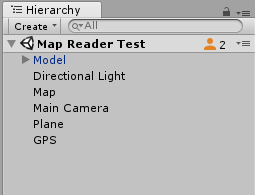
\includegraphics[scale=1]{hierarchy}
	\caption{Hierarchy window}
\end{figure}
\subsubsection{Inspector Window}
The inspector window works closely with the hierarchy window in that it shows all the properties of objects in the scene and which can all be adjusted and tweaked. You can add components to objects such as scripts which control the logic of that object. To advance this you can also change values of variables in the scripts you've created to easier fine tune what values work. It is also used to create materials for surfaces and can be used as a preview to see the code for a script without needing to open Visual Studio. \cite{Unity}
\begin{figure}[h]
	\centering
	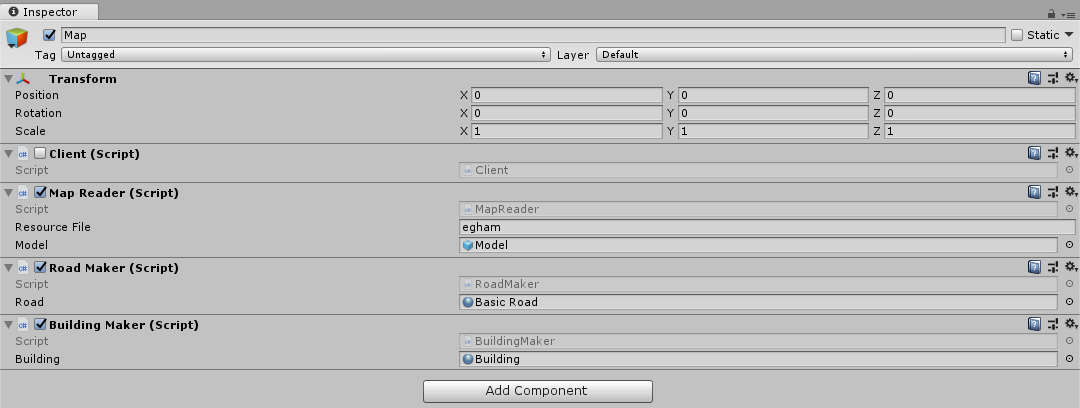
\includegraphics[scale=0.55]{inspector}
	\caption{Inspector window}
\end{figure}
\subsubsection{The Project Window}
The project window shows the file structure of the project where you can create folders and files that need to be in the game. Common practice is to separate Art, scripts, scenes etc. into different directories to keep it easy to understand and navigate.
\begin{figure}[h]
	\centering
	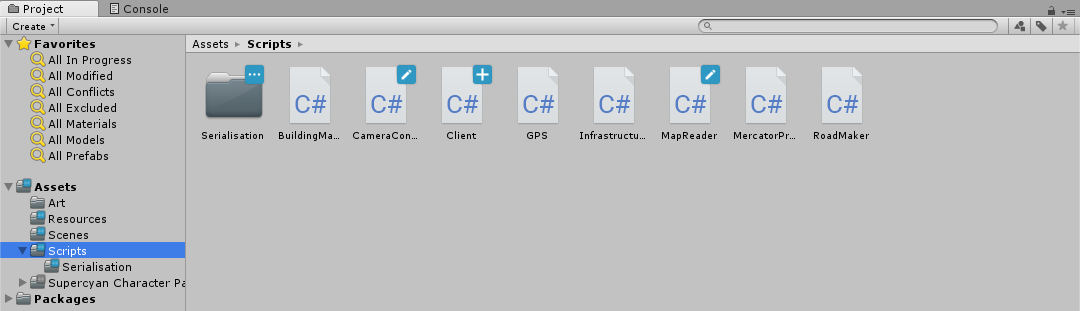
\includegraphics[scale=0.55]{project}
	\caption{Project Window}
\end{figure}
\subsection{C\# and Game Objects}
The programming aspect of Unity uses C\# scripts that are attached to game objects which can control the logic of that object. C\# is not naturally a scripting language as it is compiled before the code upon runtime. This is because the Mono framework compiles the C\# scripts and allows it to be used as a scripting language. \cite{Mono}
\\\\
Unity is closely tied to Visual Studio and so this is the IDE I am using throughout the project. Each Unity script must extend the base class MonoBehaviour as all Unity scripts are derived from this class. This base class is used to control the game loop with functions such as Start() and Update().  
\\\\
The Start() function is run once when the script begins and can be used to initiate variables and set up a game object. For example, I use this to set up the camera object behind the model at a fixed angle and distance in my camera script to lock the camera angle in place.
\\\\
The Update() method is run once every game loop and is used to update what needs to be rendered. For example, as my model moves in the game the camera also needs to update its position according to the new location of the model. More specifically, I used the method LateUpdate() for updating the position of the camera as LateUpdate() runs after all Update() methods have been run first. It ensures that all the game objects have been adjusted before the camera updates and renders the frame. \cite{Unity}

\subsection{Conclusion}
Described above are some of the main features I thought were most important for my learning and understanding of game development, thus why I chose to use Unity for my project. Compared to other software like Unreal Engine, it is more user-friendly allowing beginners to make a start in game developing with powerful tools. The learning resources were more abundant for Unity compared to other engines due to its popularity with beginners.

\section{Design Patterns}
There are many patterns that are used specifically for games to optimise performance and keep code readable. I am going to investigate some game patterns that will prove useful in my game. 

\subsection{Game Loop}
The game loop is the foundation of nearly all games used with the intent of decoupling game progression from user input and processor speed. It allows the game to run in its own time without having to wait for user input as this is how majority of applications are created. Animations, AI and visual effects can continue working using the game loop without input required. 
\begin{figure}[h]
	\centering
	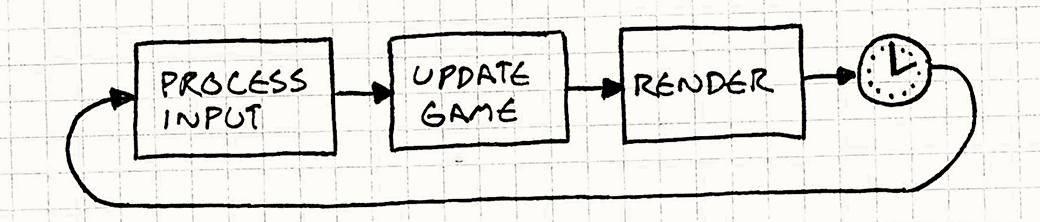
\includegraphics[scale=0.55]{game-loop-simple}
	\caption{The life cycle of a game \cite{GPP}}
\end{figure}
\\The loop carries out every frame and upon the completion of one loop, user input is processed, updates are calculated, and the output is rendered to the screen. The amount of time it takes for a loop to be completed dictates how fast the game world runs represented by a number called frames per second (FPS). More complex code or slower hardware can cause the FPS to decrease making games stutter whereas the higher FPS makes the gameplay smoother. Consequently, the aim is to write efficient code so that they run better on slow and fast systems. \cite{GPP}
\subsection{Flyweight}
Flyweight aims at reducing the number of computations the GPU must process when rendering objects that are very similar. For example, in my game, the map data needs to be processed to create hundreds of game objects which represents the roads and buildings on the map.
\\\\
To optimise this process, with flyweight, I can look at all the similarities between all the road objects. I can take all the variables that will remain the same for each road object such as material and mesh and extract it into its own class. This uses less memory as I am no longer creating the same data for many road objects but instead referencing this shared model for a road.
\\\\
However, this reduces the amount of memory that is used and not how much data the GPU processes. I need to be able to send this model of the road to the GPU once and subsequently tell it to use this model for all  future roads; this is called instanced rendering. Flyweight works well with the factory design pattern to make sure new objects are only created if a different variety road is required, else I can use the previously created objects, lessening the data usage. \cite{GPP}
\pagebreak
\subsection{Factory}
The factory pattern defines an interface for creating an object but allows the implemented classes to decide which class to instantiate. It replaces class constructors by abstracting the process of object creation so that the type of class to be generated can be decided at runtime. \cite{GOF}
\\\\
An example of this is, that could apply to my game, is in the loot system. When defeating an enemy and obtaining a piece of loot, the item can be decided at runtime based on the character class and level. Certain classes will use certain weapons therefore only that specific weapon should be available as loot for that class. \cite{Factory}

\subsection{Singleton}
The motive of the singleton pattern is to be able to have one instance of a class that has a global point of access to it. There are situations where having more than one instance of a class can cause issues due to its functionality. 
\\\\
In my game, I need to use the GPS location services to retrieve the latitude and longitude for the user's location. Having one instance of the GPS means that there is no way another instance could be made, where different coordinates could conflict causing the player model to move frantically around the screen. \cite{GOF}
\\\\
I also need these coordinates in different areas in my game ranging from map generation, model positioning and client-server communication. Each of these areas cannot make their own instance of the GPS for the reasons described above, therefore, singleton provides a global point of access. \cite{GPP}

\subsection{Observer}
Throughout gameplay, events will be to triggered if some certain criteria are met and it is not logical to embed these events throughout the code base. I can use the observer pattern to decouple these systems making sure each system knows as little as possible about the other. 
\\\\
This ideology can be used in my game when making enemies appear on the screen. Ideally, enemies should not show up on the screen if the user is not within the radius of the enemy. The observer pattern can help me to keep an eye on the user’s location and whether they are close enough to an enemy for it to be rendered. Once the user is close enough, the GPS system will send a notify signal for the observer to see. When the observer sees this, it can act upon this data by rendering the enemy to the screen.
\begin{figure}[h]
	\centering
	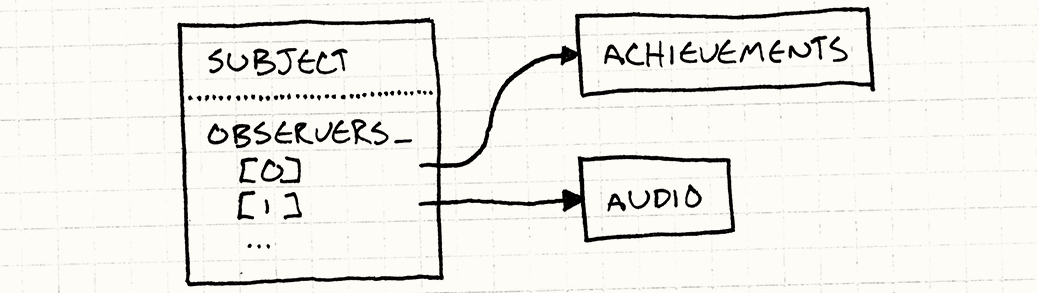
\includegraphics[scale=0.55]{observer-list}
	\caption{A subject with a list of objects \cite{GPP}}
\end{figure}
\\\\
I can create a subject class which contains all the observers that need to be notified for different aspects of the game such as an audio system, so that the correct sounds can be played at the right time. Whenever a notification is made the observers will be made known to it and the corresponding one will carry out its function. \cite{GPP}

\section{OpenStreetMap}
A vital feature of the game is for the user to be able to view their location on a map that updates as they move around in the real world. This feature is what will make the game immersive and fun, therefore, needs to be implemented correctly. I decided to use OpenStreetMap data as it is free and open source giving me a lot more control in how to present this data to the user compared to software like Google Maps. I learnt the following using a tutorial and code from the Sloan Kelly YouTube channel. \cite{Sloan}

\subsection{Map Data}
The map data can be downloaded from the OpenStreetMap API using HTTP requests that take a boundary outlining the longitude and latitude. It essentially outlines a rectangle and all the map data within the rectangle is returned to the client. \cite{API}
\\\\
My initial testing has been with a text file, containing XML map data, I downloaded from OpenStreetMap of the local Egham area and I mainly focused on being able to parse this information and creating a map from the data. At the top of the file, the boundary latitudes and longitudes that outline the map data are stored. The rest of the data are one of three elements; nodes, ways or relations. The most important elements for my project are the nodes and ways elements as they contain the map data.
\\\\
The nodes represent points in space and are represented with a node tag(“<node>”) in the text document. They contain a latitude and longitude as well as the time the node was created and the user who created it. A node could represent a park bench, a statue or another point of interest. \cite{API}
\begin{figure}[h]
	\centering
	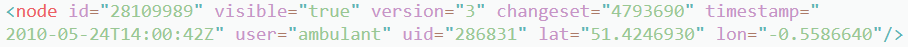
\includegraphics[scale=0.64]{node}
	\caption{A node tag in an OpenStreetMap file}
\end{figure}
\\A "way" represents a set of nodes that create a road or a building. These nodes are used to create a path from point A to B allowing me to map the data. Buildings can be separated from roads if the first node in the list is equal to the last node in the list. This tells me that the way finishes where it starts and is a building rather than a road. Other information is stored in each way such as building names, building height and road name which I can use to portray this to the user.
\begin{figure}[h]
	\centering
	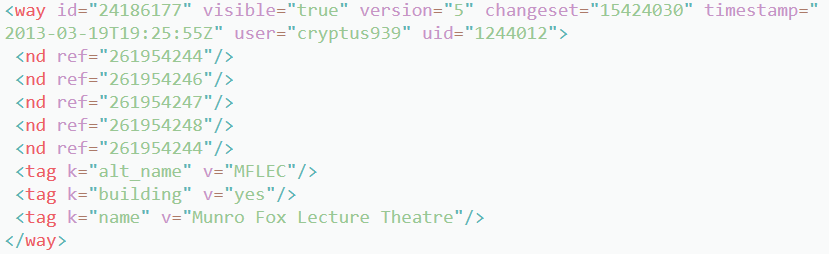
\includegraphics[scale=0.7]{way}
	\caption{A way tag in an OpenStreetMap file}
\end{figure}

\subsection{Processing the Data}
To process the data text file in Unity I needed to create a system that could read the data and process each element and decide what to render to the screen. I used an XML parser, included in C\#, to read each XML node in the text file and processed it depending on which element it is (node or way). I created a class for each node and way such that when the tag was read its respective object would be created containing the necessary data i.e. latitude and longitude. 
\\\\
Longitude and latitude are not useful values to me in the digital realm where vectors and coordinates are used so I needed to convert them to x and y values. To do this I used the Mercator map projection to translate these values into coordinates. I used the Mercator projection method as it is the most common map used today as it is popular for navigational uses. Each node is then stored in a dictionary using its ID to reference the data and the ways are stored in a list. 
\subsection{Drawing the Map}
After processing the data from the file, I needed to portray this data. I created two classes to create both the roads and the buildings. I begin the road class by going through all the ways data identifying those that are roads and creating new game objects for them.  
\\\\
To draw the road, we must use a MeshFilter and MeshRenderer to create an area to be filled with a specified material. A mesh is like an invisible surface that is created using triangles which are each formed using vectors. For each way, four vectors were created to represent the rectangular shape of the road.  
\\\\
The rectangle is then split into two triangles by splitting the rectangle diagonally. The vectors for each triangle are stored in a list in the MeshFilter previously created so that each triangle can be drawn with a specified material. The outcome can be seen in Fig. 3 showing Royal Holloway.
\\\\
A similar process is used to create the walls for a building but instead of using a flat rectangle where its height equalled zero, the rectangle is given a height according to map data. This creates a 3D effect where the buildings stand out more. 

\subsection{Real time Map Updates}
With the current method used to draw the map data, if the user walks out of the boundaries of the text file, there is no more map data to draw as there is no data for that location. To update this the client needs to connect to the OpenStreetMap API using an HTTP GET request to download a new text file containing more data about the new whereabouts.
\\\\
Also, as it stands the current text file is quite large and can take some time to load all the data and render all the roads and buildings. To fix both issues, the client will download new map data from OpenStreetMap whenever the user gets close to a boundary. The client will create a boundary based on the current GPS location and send this to the API server to get the new text file. All the new data will be processed real-time and any new roads or buildings will be processed and rendered.

\subsection{Conclusion}
By using OpenStreetMap I have learnt a lot about how map-data is processed in order for it to become the familiar map that we are all used to using. I had to manage the raw data and create a real map from it which has given me a lot of options for how I feel the map should be displayed in my game. For example, I could change the map projection that is used to create a different type of map or customise the materials that the roads and buildings are made from. 

\section{Proof of Concepts}
These are the proof of concept programs that I have created to show that I can create some of the fundamental features of the game I wish to create. These are the essential parts of the game which provide the pillar upon which the rest of the game is built.
\\\\
I did not use traditional Test-Driven Design (TDD) when creating these programs as I felt it would have slowed my learning process of a new technology. I used these programs to help me learn about Unity and the use of OpenStreetMap to further develop my understanding. It was not possible at the beginning to begin unit testing when I did not know what I would be testing. Moving forward I intend to use TDD where I will recreate these proofs of concepts with my better knowledge and comprehension.
\\\\
To store my projects, I used SVN version control as well as a built-in Unity feature that allows me to store projects on the cloud. This allowed me to work on features across multiple machines without having to commit an unfinished feature or non-functional code. Once I finished a feature, I would commit this to the SVN repository. 
\\\\
I worked on multiple projects at once containing different proof of concepts and once completed added these features to one project. This helped me focus on different aspects of the project and solidify my comprehension before integrating these features into one project.

\subsection{Creating the Map}
To gain a better understanding of how the OpenStreetMap map data works I watched a tutorial and used online code to complete this program. This program was one of the larger concept programs as I had to process and categorise a lot of data. This UML shows the different classes and how they interacted with each other. \cite{Sloan}
\begin{figure}[h]
	\includegraphics[scale=0.35]{"Map UML"}
	\label{Figure 2: UML of processing map}
	\caption{UML of the map generation system}
\end{figure}
\\Below is the main script that is used to create a dictionary of nodes and a list of nodes from the text file. I created a class for bounds, nodes and ways which respectively hold; the map boundaries, a node with its coordinates and a list of nodes making a path. So, for each XmlNode in the text file that has the tag “<node>” a corresponding OsmNode object was created with the relevant data and this object was added to the dictionary of nodes above. The Boolean value at the end dictates when the road and building renderers can begin as all the data has been read and processed. 
\pagebreak
\begin{Verbatim}[tabsize=4]
void Start () {
	nodes = new Dictionary<ulong, OsmNode>();
	ways = new List<OsmWay>();
	var txtAsset = Resources.Load<TextAsset>(resourceFile);
	XmlDocument doc = new XmlDocument();
	doc.LoadXml(txtAsset.text);
	
	SetBounds(doc.SelectSingleNode("/osm/bounds"));
	GetNodes(doc.SelectNodes("/osm/node"));
	GetWays(doc.SelectNodes("/osm/way"));
	IsReady = true;
}
\end{Verbatim}

\subsection{GPS Location}
The model in the game needs to be mapped correctly to the location of the user in real life, therefore the users' longitude and latitude are required. The GPS instance uses the singleton design pattern as I don’t want there to be multiple instances of the GPS to be running and it makes this data accessible to all my classes. 
\\\\
In this class, I use a coroutine that initiates the GPS location service making sure that the user is asked for GPS to be used. A coroutine lets me start a function I have created that can run on its own timer outside of the game loop. Normally, the Update() function is used for game updates, which is called every frame. Here I want to wait twenty seconds for the user to enable GPS before concluding that GPS is not enabled. 
\\\\
When I have concluded the state of the GPS I can break out of the function; the key word here is "yield". "yield return" will make the coroutine pause and as the game loops, it will be resumed in the frame where one second has passed. “Yield break” will break out of the function as the state of the GPS has been resolved. The function of a coroutine is of return type IEnumerator as either null is returned by use of “yield break” or an IEnumerator object is returned, “new WaitForSeconds(1)”. \cite{Unity} \cite{GPS}
\begin{Verbatim}[tabsize=4]
private IEnumerator StartLocationService() {
	if (!Input.location.isEnabledByUser) {
		Debug.Log("User not enabled GPS");
		yield break;
	}
	
	Input.location.Start();
	int maxWait = 20;
	
	while (Input.location.status == LocationServiceStatus.Initializing && maxWait>0){
		yield return new WaitForSeconds(1);
		maxWait--;
	}
	
	if (maxWait <= 0) {
		Debug.Log("Timed Out!");
		yield break;
	}
	
	if (Input.location.status == LocationServiceStatus.Failed) {
		Debug.Log("Unable to determine device location");
		yield break;
	}
	
	Update();
	yield break;
}
\end{Verbatim}

\subsection{Server - Client Connection}
The foundation of the server is that it needs to work with multiple clients because in future I intend to have multiple players interacting with each other. To handle this, I found that I needed to use an asynchronous server which uses asynchronous sockets meaning that the server would not be suspended whilst waiting for a client to connect. As well as this the client is built similarly so the execution of the client application is not suspended whilst it is waiting for the server to respond.
\\\\
As it stands the client and server only share a string upon connection and doesn’t have any game functionality yet. It is intended to communicate data and shared resources between multiple clients for multiplayer such as user info and status.
\\\\
Like a normal socket server, both the client needs to know the IP address and port of the socket they will be exchanging data in. The difference is in the use of a special variable type called ManualResetEvent which are used in a similar way as semaphores are used in OS scheduling. It is needed so that the main threads of an application can run without waiting for client/server responses. \cite{MRE}
\\\\
When a client connects the main thread can continue waiting for other clients to connect whilst also serving the current client at the same time. The socket listener will wait for a client to connect triggering the AcceptCallback() method which subsequently signals the ManualResetEvent variable (allDone), allowing the main thread to continue waiting for new connections immediately. \cite{Server} 

\begin{Verbatim}[tabsize=4]
	try {
		listener.Bind(localEndPoint);
		listener.Listen(100);
		while (true) {
			// Set the event to nonsignaled state.
			allDone.Reset();
			
			// Start an asynchronous socket to listen for connections.
			Console.WriteLine("Waiting for a connection...");
			listener.BeginAccept( 
			new AsyncCallback(AcceptCallback), listener);
			
			// Wait until a connection is made before continuing.
			allDone.WaitOne();
		}
	} catch (Exception e) {
		Console.WriteLine(e.ToString());
	}
	Console.WriteLine("\nPress ENTER to continue...");
	Console.Read();
}
public static void AcceptCallback(IAsyncResult ar) {
	// Signal the main thread to continue.
	allDone.Set();	
	// Get the socket that handles the client request.
	Socket listener = (Socket) ar.AsyncState;
	Socket handler = listener.EndAccept(ar);
	
	// Create the state object.
	StateObject state = new StateObject();
	state.workSocket = handler;
	handler.BeginReceive( state.buffer, 0, StateObject.BufferSize, 0,
	new AsyncCallback(ReadCallback), state);
}
\end{Verbatim}

\subsection{Camera Movement}
Although I could have used the easy method of making the camera object a child of the model object, I felt that the viewing angles created were not right for the game. I decided to configure the vector location of the camera dependent on the model’s location whilst also adding some touch controls so that the camera could pivot around the model.
\\\\
The model is placed on the map based on GPS location, therefore, I could use this as a reference point for where the camera should be positioned. I began making the camera position equal to the model's position and adjusted these values. As the camera will be in a fixed position, I tinkered with values adjusting the height and distance from the model to create a pleasant viewing angle.
\\\\ 
The model’s vector is going to change every update meaning the camera should adjust accordingly. I stored the vector between the camera and the model in the Start() function so that this offset can be applied every frame no matter of the model’s new vector. The new vector plus the offset I calculated will always give the correct viewing angle. I also detected for touch input such that when the user swipes their finger across the screen, the viewing angle changes on the horizontal axis.
\begin{Verbatim}[tabsize=4]
private void Start() {
	cameraPosition = model.transform.position;
	cameraPosition[1] += 80;
	cameraPosition[2] -= 100;
	offset = cameraPosition - model.transform.position;
	transform.position = cameraPosition;
	UpdateCamera();
}
private void LateUpdate() {
	if (Input.touchCount > 0 && Input.GetTouch(0).phase == TouchPhase.Moved) {
		offset = Quaternion.AngleAxis(Input.GetAxis("Mouse X") * SPEED, Vector3.up) * offset;
	}
	transform.position = model.transform.position + offset;
	UpdateCamera();
}
\end{Verbatim}
\section{Project Diary}
\subsection{September}
My focus this month was to learn how to use Unity and to program in C\# by learning from tutorials and making practice programs. I managed to stick to this plan and found it beneficial before tackling the project at hand.
\subsection{October}
After learning the fundamentals of Unity, I moved my focus to OpenStreetMap as this was another large part of the project. Using an online tutorial, I successfully recreated the local Egham area in my game. I also finished a project where I could get the GPS coordinates of a user’s location.
\subsection{November}
After the first two successful months, my progress began to slow as I got caught up with bugs about the camera position and creating the battle system. I eventually decided that I needed to make the foundation of the games system work, including client-server before continuing with game logic. With better time management I could have avoided this halt in progress by better understanding my goals for the first term.
\subsection{December}
As all my proof of concepts were finished, I used this time to focus on other work such as the interim report. I also refactored my code making sure to remove dead code and improve efficiency.
\bibliographystyle{plain}
\bibliography{references}

\end{document}          
